\documentclass{scrartcl}

\usepackage{graphicx}
\usepackage[utf8]{inputenc}
\usepackage[T1]{fontenc}
\usepackage[english]{babel}
\usepackage{amsmath}
\usepackage{mathtools}
\usepackage{amssymb}
\usepackage{amsthm}
\usepackage{listings}
\usepackage{stmaryrd}
\usepackage[style=english]{csquotes}
\usepackage[language=english, backend=biber, style=alphabetic, sorting=nyt]{biblatex}
\usepackage{tikz}

\addbibresource{bibliography.bib}

\title{Miniproject - Algebraic Geometry}
\author{Simon Pohmann}
\date{}

\newcommand{\R}{\mathbb{R}}
\newcommand{\N}{\mathbb{N}}
\newcommand{\Z}{\mathbb{Z}}
\newcommand{\Q}{\mathbb{Q}}
\newcommand{\C}{\mathbb{C}}
\newcommand{\I}{\mathbb{I}}
\newcommand{\V}{\mathbb{V}}
\newcommand{\Proj}{\mathbb{P}}
\newcommand{\Aff}{\mathbb{A}}
\newcommand{\GL}{\mathrm{GL}}
\newcommand{\Gr}{\mathrm{Gr}}
\newcommand{\sgn}{\mathrm{sgn}}
\newcommand{\contradiction}{\text{contradiction}}
\newcommand{\extpow}{\mathchoice{{\textstyle\bigwedge}}
    {{\bigwedge}}
    {{\textstyle\wedge}}
    {{\scriptstyle\wedge}}}
\newcommand{\vspan}{\mathrm{span}}
\newcommand{\divides}{\ | \ }
\newcommand\restr[2]{{
    \left.\kern-\nulldelimiterspace
    #1
    \vphantom{\big|}
    \right|_{#2}
}}

\theoremstyle{definition}
\newtheorem{definition}[subsection]{Definition}
\newtheorem{remark}[subsection]{Remark}
\newtheorem{lemma}[subsection]{Lemma}
\newtheorem{example}[subsection]{Example}
\newtheorem{proposition}[subsection]{Proposition}
\newtheorem{corollary}[subsection]{Corollary}
\newtheorem{theorem}[subsection]{Theorem}

\begin{document}
\maketitle

For this document, let $V$ be a finitely dimensional vector space with basis $B = (b_1, ..., b_n)$.

\section{Part I}
First of all, I will include here a more formal definition of the exterior product, which is required for rigorous proofs later on.
\begin{definition}
    Define the $d$-th exterior power of $V$ as a quotient of the free vector space of $B \times ... \times B$ as follows
    \begin{align*}
        \extpow^d V := \mathrm{Fr}\Bigl(\bigtimes_{i = 1}^d B\Bigr) \ \bigm/ \ U
    \end{align*}
    where
    \begin{align*}
        U = \vspan \bigl\{ (v_1, ..., v_d) + (v_1, ..., v_{i - 1}, v_{i + 1}, v_i, v_{i + 2}, ..., v_d) \ \bigm| \ v_1, ..., v_d \in B, 1 \leq i < d \bigr\}
    \end{align*}
    Consider also the map
    \begin{equation*}
        \wedge: \bigtimes_{i = 1}^d V \to \extpow^d V, \quad \Bigl( \sum_{i = 1}^n \lambda_{1i} b_i, ..., \sum_{i = 1}^n \lambda_{di} b_i \Bigr) \mapsto \sum_{1 \leq i_1, ..., i_d \leq n} \lambda_{1i_1} ... \lambda_{di_d} (b_{i_1}, ..., b_{i_d})
    \end{equation*}
    and use the notation $v_1 \wedge ... \wedge v_d$ to denote the image of $(v_1, ..., v_d)$ under this map.
\end{definition}
First of all, we show some basic properties of the exterior product.
It is straightforward to see that the exterior product is multilinear, i.e. $v_1 \wedge ... \wedge (v_i + v'_i) \wedge ... \wedge v_d = (v_1 \wedge ... \wedge v_d) + (v_1 \wedge ... \wedge v'_i \wedge ... \wedge v_d)$.
More interesting are the following properties.
\begin{lemma}
    \label{prop:basic_properties_exterior_product}
    Let $v_1, ..., v_d \in V$. Have for $\pi \in S_d$ that
    \begin{equation*}
        v_{\pi(1)} \wedge ... \wedge v_{\pi(k)} = \sgn(\pi) (v_1 \wedge ... \wedge v_d)
    \end{equation*}
    Furthermore if $v_i = v_j$ for some $i \neq j$, then
    \begin{equation*}
        v_1 \wedge ... \wedge v_d = 0
    \end{equation*}
\end{lemma}
\begin{proof}
    Clearly the vectors $b_{i_1} \wedge ... \wedge b_{i_d}$ span $\extpow^d V$.
    So let
    \begin{equation*}
        u = \sum_{i_1, ..., i_{j - 1}} \lambda_{i_1, ..., i_{j - 1}} (b_1 \wedge ... \wedge b_{j - 1}), \quad w = \sum_{i_1, ..., i_{d - j - 1}} \mu_{i_1, ..., i_d} (b_{i_1} \wedge ... \wedge b_{d - j - 1})
    \end{equation*}
    be arbitrary vectors in $\extpow^{j - 1} V$ resp. $\extpow^{d - j - 1} V$ for some $1 \leq j \leq d - 1$.
    Note that for $v = \sum \tau_i b_i, v' = \sum \tau'_i b_i \in V$ have then
    \begin{align*}
        &(u \wedge v \wedge v' \wedge w) + (u \wedge v' \wedge v \wedge w) = \sum_{i_1, ..., i_{j - 1}, i_{j + 2}, ..., i_d} \quad \sum_{0 \leq i, i' \leq n} \lambda_{i_1, ..., i_{j - 1}} \mu_{i_{j + 2}, ..., i_d} \tau_i \tau'_{i'} \\
        &\Bigl(\underbrace{\bigl( b_{i_1} \wedge ... \wedge b_{i_j} \wedge b_{i_{j + 1}} \wedge ... \wedge b_{i_d}\bigr) + \bigl( b_{i_1} \wedge ... \wedge b_{i_{j - 1}} \wedge b_{i_{j + 1}} \wedge b_{i_j} \wedge b_{i_{j + 2}} \wedge ... \wedge b_{i_d} \bigr)}_{= 0 \ \text{as it is an element of the space $U$}} \Bigl) \\
        &= 0
    \end{align*}
    for all $u \in \extpow^{i - 1}(V), w \in \extpow^{(d - i - 1)}(V)$.
    Hence
    \begin{equation*}
        u \wedge v \wedge v' \wedge w = -(u \wedge v' \wedge v \wedge w)
    \end{equation*}

    Every $\pi \in S_d$ has a decomposition $\pi = \xi_1 ... \xi_n$ into transpositions $\xi_i$.
    Applying this inductively, we find that
    \begin{equation*}
        v_1 \wedge ... \wedge v_d = \sgn(\xi_i ... \xi_n) (v_{(\xi_i ... \xi_n)(1)} \wedge ... v_{(\xi_i ... \xi_n)(k)})
    \end{equation*}
    and so
    \begin{equation*}
        v_1 \wedge ... \wedge v_d = \sgn(\pi) (v_{\pi(1)} \wedge ... \wedge v_{\pi(k)})
    \end{equation*}

    Furthermore, we find that
    \begin{equation*}
        u \wedge v \wedge v \wedge w = -(u \wedge v \wedge v \wedge w) = 0
    \end{equation*}
    must be zero.
    Hence, if $v_1, ..., v_d \in V$ with $v_i = v_j$ for some $i \neq j$, then there is a permutation $\pi \in S_d$ with $\pi(1) = i, \pi(2) = j$ and
    \begin{equation*}
        v_1 \wedge ... \wedge v_d = (\sgn(\pi))(v_i \wedge v_j \wedge v_{\pi(3)} \wedge ... \wedge v_{\pi(k)}) = \sgn(\pi) 0 = 0
    \end{equation*}
\end{proof}

\begin{lemma}[Question (a)]
    Let $\dim(V) \leq 3$. Then every element of $\extpow^k(V)$ is decomposable.
\end{lemma}
\begin{proof}
    Now let $v_1, v_2, v_3$ be a set of generators of $V$.
    Consider $u_1 = \sum \lambda_i v_i, u_2 = \sum_i \mu_i v_i, u_3 = \sum_i \rho_i v_i$.
    Then by applying Lemma~\ref{prop:basic_properties_exterior_product}, we see that 
    \begin{align*}
        u_1 \wedge u_2 =& \sum_{i, j} \ \lambda_i \mu_j (\underbrace{v_i \wedge v_j}_{\mathclap{\text{$= 0$ if $i = j$}}}) = \sum_{i < j} \lambda_i \mu_j (v_i \wedge v_j) - \sum_{i > j} \lambda_i \mu_j (v_i \wedge v_j) \\
        =& \sum_{i < j} (\lambda_i \mu_j - \lambda_j \mu_i)(v_i \wedge v_j) = \alpha (v_1 \wedge v_2) + \beta (v_1 \wedge v_3) + \gamma (v_2 \wedge v_3) \\
        =& \begin{cases}
            \beta v_1 + \gamma v_2 \wedge \frac \alpha \beta v_2 + v_3 & \text{if $\beta \neq 0$} \\
            \alpha v_1 - \gamma v_3 \wedge v_2 & \text{otherwise}
        \end{cases}
    \end{align*}
    and
    \begin{align*}
        u_1 \wedge u_2 \wedge u_3 =& \sum_{i, j, l} \ \lambda_i \mu_j \rho_l (\underbrace{v_i \wedge v_j \wedge v_l}_{\mathclap{\text{$= 0$ unless $i, j, l$ pairwise distinct}}}) \\
        =& \sum_{\pi \in S_3} \lambda_{\pi(1)} \mu_{\pi(2)} \rho_{\pi(3)} (v_{\pi(1)} \wedge v_{\pi(2)} \wedge v_{\pi(3)}) \\
        =& \sum_{\pi \in S_3} \lambda_{\pi(1)} \mu_{\pi(2)} \rho_{\pi(3)} \sgn(\pi) (v_1 \wedge v_2 \wedge v_3) \\
        =& (v_1 \wedge v_2 \wedge v_3) \sum_{\pi \in S_3} \lambda_{\pi(1)} \mu_{\pi(2)} \rho_{\pi(3)} \sgn(\pi)
    \end{align*}
    are decomposable.
    Further, it is easy to see from Lemma~\ref{prop:basic_properties_exterior_product} that $\extpow^k(V) = \{ 0 \}$ for $k \geq 4$, which is trivially decomposable.
\end{proof}

\begin{example}[Question (b)]
    Consider $V = k^4$. 
    Then the element $w := (e_1 \wedge e_2) + (e_3 \wedge e_4) \in \extpow^2(V)$ is not decomposable. 
\end{example}
\begin{proof}
    Assume it was, then there are $a, b \in k^4$ such that
    \begin{equation*}
        w = \sum_i a_i e_i \wedge \sum_j b_j e_j = \sum_{i < j} (a_i b_j - a_j b_i) (e_i \wedge e_j)
    \end{equation*}
    In other words
    \begin{equation*}
        a_1b_2 - a_2b_1 = 1, \ a_3b_4 - a_4b_3 = 1, \ a_i b_j - a_j b_i = 0 \ \text{for all $(i, j) \neq (1, 2), (3, 4)$}
    \end{equation*}
    Clearly $a_1 b_2 \neq 0$ or $a_2 b_1 \neq 0$.
    Similarly, have $a_3 b_4 \neq 0$ or $a_4 b_3 \neq 0$.
    As all expressions are symmetric w.r.t swapping $a_1, b_2$ with $a_2, b_1$ and $a_3, b_4$ with $a_4, b_3$, we may assume wlog that $a_1 b_2, a_3 b_4 \neq 0$.

    Have $a_1 b_4 = a_4 b_1$ and $a_2 b_4 = a_4 b_2$.
    We know that $a_1 b_4 \neq 0$ and so
    \begin{equation*}
        \frac {a_2} {a_1} = \frac {a_2 b_4} {a_1 b_4} = \frac {a_4 b_2} {a_4 b_1} = \frac {b_2} {b_1} \ \Rightarrow \ a_2 b_1 = a_1 b_2
    \end{equation*}
    This contradicts $a_1 b_2 - a_2 b_1 = 1$.
\end{proof}
For the next parts of the mini project, we first need more basic properties of the exterior product.
\begin{lemma}
    \label{prop:linear_transform_extpow}
    Let $A = (a_{ij}) \in \GL_d(k)$ and $v_1, ..., v_d \in V$.
    Then
    \begin{equation*}
        \Bigl( \sum_j a_{1j}v_j \Bigl) \wedge ... \wedge \Bigl( \sum_{j} a_{dj} v_j \Bigr) = \det(A) (v_1 \wedge ... \wedge v_d)
    \end{equation*}
\end{lemma}
\begin{proof}
    By a direct computation using Lemma~\ref{prop:basic_properties_exterior_product}, we find
    \begin{align*}
        &\Bigl( \sum_j a_{ij} v_j \Bigr) \wedge ... \wedge \Bigl( \sum_j a_{dj} v_j \Bigr) = \sum_{j_1, ..., j_d} a_{1j_1} ... a_{dj_d} (v_{j_1} \wedge ... \wedge v_{j_d}) \\
        = &\sum_{\pi \in S_d} a_{1\pi(1)} ... a_{d\pi(d)} (v_{\pi(1)} \wedge ... \wedge v_{\pi(d)}) \\
        = &\sum_{\pi \in S_d} a_{1\pi(1)} ... a_{d\pi(d)} \sgn(\pi) (v_1 \wedge ... \wedge v_d) \\
        = &(v_1 \wedge ... \wedge v_d) \ \sum_{\pi \in S_d} \sgn(\pi) \prod_{j = 1}^d a_{j\pi(j)} = \det(A) (v_1 \wedge ... \wedge v_d)
    \end{align*}
    where the last equality holds due to the Leibniz determinant formula.
\end{proof}
The next two lemmas are quite fundamental, as they can be used as a basic tool to prove linear independence in the exterior product.
\begin{lemma}
    \label{prop:basis_product_independence}
    The vectors $b_{i_1} \wedge ... \wedge b_{i_d}$ for $i_1 < ... < i_d$ form a basis of $\extpow^d V$.
\end{lemma}
\begin{proof}
    This proof is slightly technical, as I wanted to provide a rigorous proof using only the definition of $\extpow^d V$ and some properties of the symmetric group $S_d$.
    The core idea is to show the linear independence by going to down to the free product underlying $\extpow^d V$, and then show that we cannot use the vectors $(b_{i_1}, ..., b_{i_d}) + (b_{i_1}, ..., b_{i_{j + 1}}, b_{i_j}, ..., i_d)$ to create a nontrivial linear combination.
    Namely, assuming we have such a nontrivial linear combination, we can group it into the part where the order of the $i_1, ..., i_d$ has even/odd parity.
    The vectors with $i_1 < ... < i_d$ clearly are all on one side, and from this we can derive the claim.

    Note that by definition, the vectors $b_{i_1} \wedge ... \wedge b_{i_d}$ for any $1 \leq i_1, ..., i_d \leq n$ span $\extpow^d V$.
    By Lemma~\ref{prop:basic_properties_exterior_product}, we can rewrite any of them (that is nonzero) to be of the above form, so clearly the $b_{i_1} \wedge ... \wedge b_{i_d}$ for $i_1 < ... < i_d$ span $\extpow^d V$.

    It is left to show that they are linearly independent.
    Assume
    \begin{equation*}
        \sum_{i_1 < ... < i_d} \lambda_{i_1, ..., i_d} \bigl( b_{i_1} \wedge ... \wedge b_{i_d} \bigr) = 0
    \end{equation*}
    Then clearly
    \begin{equation*}
        \sum_{i_1 < ... < i_d} \lambda_{i_1, ..., i_d} \bigl( b_{i_1}, ..., b_{i_d} \bigr) \in U
    \end{equation*}
    where $U$ is the vector space from the definition of $\extpow^d V$.
    So
    \begin{align*}
        \sum_{i_1 < ... < i_d} \lambda_{i_1, ..., i_d} \bigl( b_{i_1}, ..., b_{i_d} \bigr) = &\sum_{j, \ i_1, ..., i_d} \mu_{j, i_1, ..., i_d} \\
        &\Bigl( \bigl( b_{i_1}, ..., b_{i_d} \bigr) + \bigl( b_{i_1}, ..., b_{i_{j - 1}}, b_{i_{j + 1}}, b_{i_j}, b_{i_{j + 2}}, ..., b_{i_d} \bigr) \Bigr)
    \end{align*}
    Note that we can assume wlog that the sum on the right-hand side goes only over $i_1, ..., i_d$ distinct.
    The reason is that the other vectors on the right-hand side are contained in
    \begin{equation*}
       \vspan \{ (b_{i_1}, ..., b_{i_d}) \ | \ \text{$i_1, ..., i_d$ not distinct} \}
    \end{equation*}
    which only trivially intersects the space
    \begin{equation*}
        \vspan\{ (b_{i_1}, ..., b_{i_d}) \ | \ \text{$i_1, ..., i_d$ distinct} \}
    \end{equation*}
    due to the properties of the free product (the spaces share now basis vectors).

    Now consider for $i_1, ..., i_d$ distinct the ``sorting permutation'' $\sigma_i \in S_d$, which is the unique permutation such that $i_{\sigma(1)} < ... < i_{\sigma(d)}$.
    Then
    \begin{align*}
        \sum_{i_1 < ... < i_d} \lambda_{i_1, ..., i_d} \underbrace{\bigl( b_{i_1}, ..., b_{i_d} \bigr)}_{\sgn(\sigma_i) = 1 \ \text{as} \ \sigma_i = \mathrm{id}} = &\sum_{\substack{j, \ i_1, ..., i_d\\\sgn(\sigma_i) = 1}} \underbrace{\sgn(\sigma_i) \bigl( \mu_{j, i_1, ..., i_d} - \mu_{j, i_1, ..., i_{j + 1}, i_j, ..., i_d} \bigr)}_{=: \mu'_{j, i_1, ..., i_d}} \\
        &\Bigl( \bigl( b_{i_1}, ..., b_{i_d} \bigr) + \bigl( b_{i_1}, ..., b_{i_{j - 1}}, b_{i_{j + 1}}, b_{i_j}, b_{i_{j + 2}}, ..., b_{i_d} \bigr) \Bigr)
    \end{align*}
    This yields
    \begin{align*}
        &-\sum_{\substack{j, \ i_1, ..., i_d\\\sgn(\sigma_i) = 1}} \Bigl( \mu'_{j, i_1, ..., i_d} - \begin{cases}
            \lambda_{i_1, ..., i_d} & \text{if $i_1 < ... < i_d, j = 0$} \\
            0 & \text{otherwise}
        \end{cases} \Bigr) (b_{i_1}, ..., b_{i_d}) \\
        =& \sum_{\substack{j, \ i_1, ..., i_d\\\sgn(\sigma_i) = -1}} \mu'_{j, i_1, ..., i_{j + 1}, i_j, ..., i_d} (b_{i_1}, ..., b_{i_d})
    \end{align*}
    However, all vectors on the left-hand side are contained in
    \begin{equation*}
        \vspan \{(b_{i_1}, ..., b_{i_d}) \ | \ \sgn(\sigma_i) = 1 \}
    \end{equation*}
    and all vectors on the right-hand side are contained in
    \begin{equation*}
        \vspan \{(b_{i_1}, ..., b_{i_d}) \ | \ \sgn(\sigma_i) = -1 \}
    \end{equation*}
    These two spaces intersect trivially, and so find
    \begin{equation*}
        \sum_{\substack{j, \ i_1, ..., i_d\\\sgn(\sigma_i) = -1}} \mu'_{j, i_1, ..., i_{j + 1}, i_j, ..., i_d} (b_{i_1}, ..., b_{i_d}) = 0
    \end{equation*}
    Clearly the different $(b_{i_1}, ..., b_{i_d})$ are linearly independent, so find that all $\mu'_{j, i_1, ..., i_d} = 0$.
    Observe now that thus all $\lambda_{i_1, ..., i_d} = 0$ and the claim is shown.
\end{proof}
\begin{lemma}
    \label{prop:subspace_closed}
    Let $v \in V$ and $w \in \extpow^{d - 1} W$ for a linear subspace $W \leq V$. 
    If $v \wedge w \in \extpow^d W$ then $v \in W$ or $w = 0$.
    Here
    \begin{equation*}
        \extpow^d W := \{ w_1 \wedge ... \wedge w_d \ | \ w_i \in W \} \leq \extpow^d V
    \end{equation*}
    is a subspace of $\extpow^d V$.
\end{lemma}
\begin{proof}
    wlog assume that $b_1, ..., b_m$ are a basis of $U$.
    Then
    \begin{equation*}
        w = \sum_{i_1 < ... < i_{d - 1} < m} \lambda_{i_1, ..., i_{d - 1} \leq m} (b_{i_1} \wedge ... \wedge b_{i_{d - 1}})
    \end{equation*}
    So with $v = \sum_i \mu_i b_i$ get
    \begin{align*}
        v \wedge w =& \sum_{i_1 < ... < i_{d - 1} \leq m} \lambda_{i_1, ..., i_{d - 1}} (v \wedge b_{i_1} \wedge ... \wedge b_{i_{d - 1}}) \\
        =& \sum_{i_1 \leq n, \ i_1 < ... < i_{d - 1} \leq m} \mu_{i_1} \lambda_{i_2, ..., i_d} (b_{i_1} \wedge ... \wedge b_{i_d})
    \end{align*}
    By assumption, we also find
    \begin{align*}
        v \wedge w =& \sum_{i_1 < ... < i_d \leq m} \tau_{i_1, ..., i_d} (b_{i_1} \wedge ... \wedge b_{i_d})
    \end{align*}
    Both representations are equal, hence
    \begin{equation*}
        \sum_{i_1 \leq n, \ i_2 < ... < i_d \leq m} \Bigl( \mu_{i_1}\lambda_{i_2, ..., i_d} - \begin{cases}
            \tau_{i_1, ..., i_d} & \text{if $i_1 \leq m$} \\
            0 & \text{otherwise}
        \end{cases} \Bigr) (b_{i_1} \wedge ... \wedge b_{i_d}) = 0
    \end{equation*}
    Hence by the previous Lemma~\ref{prop:basis_product_independence}, we see that for all $i_2 < ... < i_d \leq m < i_1 \leq n$ have
    \begin{equation*}
        0 = \mu_{i_1}\lambda_{i_2, ..., i_d} - \begin{cases}
            \tau_{i_1, ..., i_d} & \text{if $i_1 \leq m$} \\
            0 & \text{otherwise}
        \end{cases}
    \end{equation*}
    So in particular find for all $i_2 < ... < i_d \leq m < i_1 \leq n$ that
    \begin{equation*}
        \mu_{i_1} \lambda_{i_2, ..., i_d} = 0
    \end{equation*}
    Hence either $\mu_{i_1} = 0$ for all $i_1 > m$ and so $v \in U$, or all $\lambda_{i_2, ..., i_d} = 0$ (for $i_2 < ... < i_d \leq m$) and so $w = 0$.
\end{proof}
\begin{lemma}
    \label{prop:extpow_zero_iff_independent}
    For $v_1, ..., v_d \in V$ have
    \begin{equation*}
        v_1 \wedge ... \wedge v_d = 0 \ \Leftrightarrow \ v_1, ..., v_d \ \text{linearly dependent}
    \end{equation*}
\end{lemma}
\begin{proof}
    For the direction $\Leftarrow$, assume that $v_1, ..., v_d$ are not independent. 
    Then there is a nonzero vector $a_1 \in k^d$ with $\sum a_{1i} v_i = 0$.
    Clearly, we can extend $a_1$ to a basis $a_1, ..., a_d$ of $k^d$, which gives a matrix $A = (a_{ij}) \in \GL_d(k)$.

    However by Lemma~\ref{prop:linear_transform_extpow} we now get
    \begin{align*}
        0 =& 0 \wedge \Bigl( \sum_j a_{2j} v_j \Bigr) \wedge ... \wedge \Bigl( \sum_j a_{dj} v_j \Bigr) = \Bigl( \sum_j a_{1j} v_j \Bigr) \wedge ... \wedge \Bigl( \sum_j a_{dj} v_j \Bigr) \\
        =& \det(A) (v_1 \wedge ... \wedge v_d)
    \end{align*}
    and so $v = v_1 \wedge ... \wedge v_d = 0$ as $\det(A) \neq 0$.

    For the other direction, let $v_1, ..., v_d$ be linearly independent.
    Clearly, we can extend them to a basis $v_1, ..., v_n$ of $V$.
    We then see that there is a matrix $A = (a_{ij}) \in \GL_n(k)$ with $v_i = \sum_j a_{ij} b_j$.
    So by Lemma~\ref{prop:linear_transform_extpow} have
    \begin{equation*}
        v_1 \wedge ... \wedge v_n = \underbrace{\det(A)}_{\neq 0} (b_1 \wedge ... \wedge b_n) \neq 0
    \end{equation*}
    So clearly $v_1 \wedge ... \wedge v_d \neq 0$ as $0 \wedge (v_{d + 1} \wedge ... \wedge v_n) = 0$ for all $v_{d + 1}, ..., v_n \in V$.
\end{proof}
Now we can see that in general, the exterior product contains not decomposable elements.
\begin{lemma}[Question (c)]
    \label{prop:characterization_decomposable_d_even}
    Let $d$ be even.
    An element $\omega \in \extpow^d V$ is decomposable if and only if $\omega \wedge \omega \in \extpow^{2d} V$ is zero.
\end{lemma}
\begin{proof}
    The direction $\Rightarrow$ even holds generally. Assume $\omega = v_1 \wedge ... \wedge v_d$.
    Then
    \begin{equation*}
        \omega \wedge \omega = v_1 \wedge ... \wedge v_d \wedge v_1 \wedge ... \wedge v_d = 0
    \end{equation*}
    by Lemma~\ref{prop:basic_properties_exterior_product}. 
    The other direction is more interesting.

    Let $\omega = v_1 + ... + v_t$ for linearly independent decomposable vectors $v_i \in \extpow^2 V$.
    Then
    \begin{align*}
        0 =& \omega \wedge \omega = \sum_{i, j} v_i \wedge v_j = \sum_{i < j} (v_i \wedge v_j) + (v_j \wedge v_i) \\
        =& \sum_{i < j} 2(v_i \wedge v_j) = 2\sum_i v_i \wedge \Bigl( \sum_{j > i} v_j \Bigr)
    \end{align*}
    Here we used that the reversing permutation $\bigl(1 \ 2d\bigr)\bigl(2 \ (2d - 1)\bigr)...\bigl(d \ (d + 1)\bigr) \in S_{2d}$ has even parity, i.e. $\sgn(\cdot) = 1$ (since $d$ is even).

    Now note that
    \begin{equation*}
        v_1 \wedge \Bigl( \sum_{j > 1} v_j \Bigr) = 0 \in \extpow^2 \vspan\{v_2, ..., v_t\}
    \end{equation*}
    and so $v_1 \in \vspan\{v_2, ..., v_t\}$ unless $\sum_{j > 1} v_j = 0$ by Lemma~\ref{prop:subspace_closed}.
    We assumed that the $v_i$ are linearly independent, so the former would give a contradiction.
    Hence $\sum_{j > 1} v_j = 0$ and thus $t = 1$, i.e. $\omega = v_1$ is decomposable.
\end{proof}

\section{Part II}

In this part, we want to consider the connection of exterior powers to the Grassmanian.
\begin{remark}[Question (a)]
    First of all, assume there are two bases $v_1, ..., v_d$ and $u_1, ..., u_d$ of a $d$-dimensional vector space $U$. 
    Then there exists a basis change matrix $A = (a_{ij}) \in \GL_d(k)$ with
    \begin{equation*}
        u_i = \sum_j a_{ij} v_j
    \end{equation*}
    So by Lemma~\ref{prop:linear_transform_extpow}, it follows that
    \begin{equation*}
        u_1 \wedge ... \wedge u_d = \det(A) (v_1 \wedge ... \wedge v_d)
    \end{equation*}
    As $v_1, ..., v_d$ resp. $u_1, ..., u_d$ are bases, they are linearly independent and in particular, we see that
    \begin{equation*}
        v_1 \wedge ... \wedge v_d \neq 0 \quad \text{and} \quad u_1 \wedge ... \wedge u_d \neq 0
    \end{equation*}
    by Lemma~\ref{prop:extpow_zero_iff_independent}.
    Hence they have well-defined images $[v_1 \wedge ... \wedge v_d]$ resp. $[u_1 \wedge ... \wedge u_d]$ in the projective space $\Proj(\extpow^d V)$.
    By the above, find
    \begin{equation*}
        [v_1 \wedge ... \wedge v_d] = [u_1 \wedge ... \wedge u_d]
    \end{equation*}
\end{remark}
This allows us to study the Grassmanian $\Gr(d, V)$ of a fixed vector space $V$.
\begin{definition}
    Define the map
    \begin{equation*}
        \phi: \Gr(d, V) \to \Proj(\extpow^d V), \quad \vspan\{v_1, ..., v_d\} \mapsto [v_1 \wedge ... \wedge v_d]
    \end{equation*}
    which is well-defined by Lemma~\ref{prop:linear_transform_extpow} as described above.
\end{definition}
\begin{lemma}[Question (a)]
    We have
    \begin{equation*}
        \mathrm{im}\phi = D := \{ [v] \in \Proj(\extpow^d V) \ | \ \text{$v$ decomposable}\}
    \end{equation*}
\end{lemma}
\begin{proof}
    First of all, note that the set $D$ is well-defined, as $v$ is decomposable if and only if $\lambda v$ is decomposable, for all $\lambda \in k^*$.

    By definition of $\phi$, we can directly observe that $\mathrm{im}\phi \subseteq D$.
    So consider an element $[v] \in D$.
    As $v$ is decomposable, it follows that $v = v_1 \wedge ... \wedge v_d$ for $v_i \in V$.
    Not it suffices to show that the $v_i$ are linearly independent, then clearly $\vspan\{v_1, ..., v_d\}$ is a well-defined $d$-dimensional vector subspace of $V$, thus an element of $\Gr(d, V)$.

    This follows directly from Lemma~\ref{prop:extpow_zero_iff_independent}.
\end{proof}
\begin{definition}
    Let $\Gr(d, n) := \Gr(d, k^n)$.
\end{definition}
In the lecture, we considered an embedding of $\Gr(d, n)$ into projective space given by minors of the basis matrix.
This corresponds to the following definition.
\begin{definition}
    Define the map
    \begin{align*}
        \rho: \Gr(d, n) &\to \Proj\Bigl(k^{\{1, ..., n\}^{(d)}}\Bigr) \cong \Proj^{{n \choose d} - 1}, \\
        \vspan\{v_1, ..., v_d\} &\mapsto \Bigl[ \det\left(\begin{matrix}
            v_{1i_1} & ... & v_{di_1} \\
            \vdots & \ddots & \vdots \\
            v_{1i_d} & ... & v_{di_d}
        \end{matrix}\right) \Bigr]_{\{i_1, ..., i_d\} \in \{1, ..., n\}^{(d)}}
    \end{align*}
    where $\{1, ..., n\}^{(d)} := \{ I \subset \{1, ..., n\} \ | \ \#I = d \}$ is the set of all $d$-element subsets of $\{1, ..., n\}$.
\end{definition}
\begin{lemma}
    \label{prop:isomorphism_extpow_det}
    There is a linear isomorphism
    \begin{align*}
        f: \extpow^d k^n &\to k^{\{1, ..., n\}^{(d)}}, \\
        \sum_j v_1^{(j)} \wedge ... \wedge v_d^{(j)} &\mapsto \Bigl( \sum_j \det\left(\begin{matrix}
            v_{1i_1}^{(j)} & ... & v_{di_1}^{(j)} \\
            \vdots & \ddots & \vdots \\
            v_{1i_d}^{(j)} & ... & v_{di_d}^{(j)}
        \end{matrix}\right) \Bigr)_{\{i_1, ..., i_d\} \in \{1, ..., n\}^{(d)}}
    \end{align*}
\end{lemma}
\begin{proof}
    For vectors $v_1, ..., v_d$ and $I = \{i_1, ..., i_d\} \in \{1, ..., n\}^{(d)}$ write
    \begin{equation*}
        A_I(v_1, ..., v_d) := \left(\begin{matrix*}
            v_{1i_1} & ... & v_{di_1} \\
            \vdots & \ddots & \vdots \\
            v_{1i_d} & ... & v_{di_d}
        \end{matrix*}\right)
    \end{equation*}
    First of all, we show that $f$ is well-defined.
    Clearly $f$ is well-defined on the decomposable vectors, as the determinant is negated by swapping columns.

    Now we have to show that $f$ yields the same value for different sum representations of an element of $\extpow^d V$.
    The idea is just that the determinant is linear in each column, but the details will be slightly technical.

    Assume
    \begin{equation*}
        \sum_l v_1^{(l)} \wedge ... \wedge v_d^{(l)} = \sum_{i_1 < ... < i_d} \lambda_{i_1, ..., i_d} (e_{i_1} \wedge ... \wedge e_{i_d})
    \end{equation*}
    Then clearly
    \begin{align*}
        \sum_{i_1 < ... < i_d} \lambda_{i_1, ..., i_d} \det(A_I(e_{i_1}, ..., e_{i_d})) = \sum_{i_1 < ... < i_d} \lambda_{i_1, ..., i_d} \begin{cases}
            1 & \text{if $I = \{i_1, ..., i_d\}$} \\
            0 & \text{otherwise}
        \end{cases} = \lambda_I
    \end{align*}
    So it suffices to show that for all $I = \{i_1, ..., i_d\} \in \{1, ..., n\}^{(d)}$ have
    \begin{equation*}
        \sum_l \det(A_I(v_1^{(l)}, ..., v_d^{(l)})) = \lambda_I
    \end{equation*}
    Assume that $v_j^{(l)} = \sum_i \mu_{l, j, i} e_i$. Since the determinant is linear in each column, find
    \begin{align*}
        &\sum_l \det(A_I(v_1^{(l)}, ..., v_d^{(l)})) = \sum_l \sum_{1 \leq j_1, ..., j_d \leq n} \mu_{l, 1, j_1} \cdot ... \cdot \mu_{l, d, j_d} \det(A_I(e_{j_1}, ..., e_{j_d})) \\
        =& \sum_l \sum_{j_1, ..., j_d \ \text{distinct}} \mu_{l, 1, j_1} \cdot ... \cdot \mu_{l, d, j_d} \cdot \begin{cases}
            \pm 1 & \text{if $\{j_1, ..., j_d\} = I$} \\
            0 & \text{otherwise}
        \end{cases} \\
        =& \sum_l \sum_{\pi \in S_d} \sgn(\pi) \mu_{l, 1, i_{\pi(1)}} \cdot ... \cdot \mu_{l, d, i_{\pi(d)}}
    \end{align*}
    On the other hand, observe that also $\wedge$ is multilinear (i.e. linear in each component), so
    \begin{align*}
        &\sum_l v_1^{(l)} \wedge ... \wedge v_d^{(l)} = \sum_l \sum_{1 \leq j_1, ..., j_d \leq n} \mu_{l, 1, j_1} \cdot ... \cdot \mu_{l, d, j_d} \bigl( e_{i_1} \wedge ... \wedge e_{i_d} \bigr) \\
        =& \sum_l \sum_{j_1, ..., j_d \ \text{distinct}} \mu_{l, 1, j_1} \cdot ... \cdot \mu_{l, d, j_d} \bigl( e_{i_1} \wedge ... \wedge e_{i_d} \bigr) \\
        =& \sum_l \sum_{i_1 < ... < i_d} (e_{i_1} \wedge ... \wedge e_{i_d}) \sum_{\pi \in S_d} \sgn(\pi) \mu_{l, 1, i_{\pi(1)}} \cdot ... \cdot \mu_{l, d, i_{\pi(d)}}
    \end{align*}
    By Lemma~\ref{prop:basis_product_independence} the $e_{i_1} \wedge ... \wedge e_{i_d}$ are a basis, and so we must already have that
    \begin{equation*}
        \lambda_{i_1, ..., i_d} = \sum_l \sum_{\pi \in S_d} \sgn(\pi) \mu_{l, 1, i_{\pi(1)}} \cdot ... \cdot \mu_{l, d, i_{\pi(d)}}
    \end{equation*}
    This shows the well-definedness.

    It is clear by definition that $f$ is linear, so it is left to show that it is bijective. 
    To show surjectivity, note that the $\pm e_I, I \in \{1, ..., n\}^{(d)}$ form a basis of $k^{\{1, ..., n\}^{(d)}}$.
    Clearly for $I = \{i_1, ..., i_d\}, J \in \{1, ..., n\}^{(d)}$ we have that
    \begin{equation*}
        f(e_{i_1} \wedge ... \wedge e_{i_d})_J = \det(A_J(e_{i_1}, ..., e_{i_j})) = \begin{cases}
            0 & \text{if $J \not\subseteq I$} \\
            \pm 1 & \text{if $J \subseteq I$}
        \end{cases}
    \end{equation*}
    so $f(e_{i_1} \wedge ... \wedge e_{i_d}) = e_I$ and we deduce that $\mathrm{im}f = k^{\{1, ..., k\}^{(d)}}$.

    Finally, note that
    \begin{equation*}
        e_{i_1} \wedge ... \wedge e_{i_d}
    \end{equation*}
    for $i_1 < ... < i_d$ form a basis of $\extpow^d k^n$ by Lemma~\ref{prop:basis_product_independence}.
    It follows that $\dim(\extpow^d k^n) = \dim(\Proj^{\{1, ..., n\}^{(d)}})$ and we find that $f$ is also injective.
\end{proof}
\begin{corollary}[Question (b)]
    \label{prop:image_phi}
    Let $\bar{f}: \Proj(\extpow^d k^n) \to \Proj^{{n \choose d} - 1}$ be the map $f$ from before modulo $k^*$.
    Then
    \begin{equation*}
        \rho = \bar{f} \circ \phi
    \end{equation*}
    and in particular, we see that $\phi(Gr(d, n))$ is a projective variety and isomorphic to $\rho(\Gr(d, n))$.
\end{corollary}
\begin{proposition}[Question (c)]
    The map $\phi$ is injective.
\end{proposition}
\begin{proof}
    Consider two $d$-dimensional subspaces $U, W$ of $k^n$ with $\phi(U) = \phi(W)$.
    Let $u_1, ..., u_l$ be a basis of $U \cap W$ and extend it to bases $u_1, ..., u_d$ of $U$ and $u_1, ..., u_l, w_{l + 1}, ..., w_d$ of $W$.
    As $\phi(U) = \phi(W)$, we can assume that the $u_i, w_i$ are scaled such that
    \begin{align*}
        0 =& (u_1 \wedge ... \wedge u_d) - (u_1 \wedge ... \wedge u_l \wedge w_{l + 1} \wedge ... \wedge w_d) \\
        =& u_1 \wedge ... \wedge u_l \wedge \bigl( (u_{l + 1} \wedge ... \wedge u_d) - (w_{l + 1} \wedge ... \wedge w_d) \bigr)
    \end{align*}
    By Lemma~\ref{prop:subspace_closed} we see that
    \begin{equation*}
        u_2 \wedge ... \wedge u_l \wedge \bigl( (u_{l + 1} \wedge ... \wedge u_d) - (w_{l + 1} \wedge ... \wedge w_d) \bigr) = 0
    \end{equation*}
    as $u_1 \notin \vspan\{u_2, ..., u_d, w_{l + 1}, ..., w_d\}$.
    Inductively, this argument shows that for all $2 \leq j \leq l + 1$
    \begin{equation*}
        u_j \wedge ... \wedge u_l \wedge (u_{l + 1} \wedge ... \wedge u_d) - (w_{l + 1} \wedge ... \wedge w_d) = 0
    \end{equation*}
    Hence
    \begin{equation*}
        (u_{l + 1} \wedge ... \wedge u_d) - (w_{l + 1} \wedge ... \wedge w_d) = 0
    \end{equation*}
    If $l < d$, we can now apply Lemma~\ref{prop:subspace_closed} again to see that
    \begin{equation*}
        u_{l + 1} \in \vspan\{ u_{l + 2}, ..., u_d, w_{l + 1}, ..., w_d \}
    \end{equation*}
    as $u_{l + 2} \wedge ... \wedge u_d \neq 0$ by Lemma~\ref{prop:extpow_zero_iff_independent}.
    However, this contradicts the linear independence of $u_{l + 1}, ..., u_d, w_{l + 1}, ..., w_d$.
    Hence it must be $l = d$ and so $U = W$.
\end{proof}

\section{Part III}
In this part, we want to investigate the geometric properties of the Grassmanian resp. the image of $\phi$.
In particular, we focus on the case $d = 2$, i.e. examine the variety $\Gr(2, V)$ for different finite-dimensional $V$.
To use our standard methods of Algebraic Geometry, we first introduce coordinates on $\Proj(\extpow^d k^n)$.
\begin{definition}
    Note that in the proof of Lemma~\ref{prop:basis_product_independence} it was shown that $v_{i_1} \wedge ... \wedge v_{i_d}$ for $i_1 < ... < i_d$ is a basis of $\extpow^d k^n$ if $v_1, ..., v_n$ is a basis of $V$.
    We introduce the homogeneous coordinates w.r.t. that basis, namely
    \begin{align*}
        x: \Proj(\extpow^d k^n) &\to \Proj_k^{\{1, ..., n\}^{(d)}} \cong \Proj_k^{{n \choose d} - 1}, \\
        \Bigl[ \sum_{i_1 < ... < i_d} \lambda_{i_1, ..., i_d} (v_{i_1} \wedge ... \wedge v_{i_d}) \Bigr] &\mapsto \bigl[ \lambda_{i_1, ..., i_d} \bigr]_{i_1 < ... < i_d}
    \end{align*}
    The individual coordinates will be denoted by $x_I$ for some $I \in \{1, ..., n\}^{(d)}$ or $x_{i_1, ..., i_d}$ for $i_1 < ... < i_d$.
\end{definition}
\begin{proposition}[Question (a)]
    \label{prop:equations_grassmanian_2}
    For the embedding $\phi: \Gr(2, V) \to \extpow^2 V$ we have
    \begin{equation*}
        \Gr(2, V) \cong \mathrm{im}\phi = \V(I)
    \end{equation*}
    where
    \begin{equation*}
        I := \langle x_{i, j}x_{u, v} + x_{i, v}x_{j, u} - x_{i, u}x_{j, v} \ | \ i < j < u < v \rangle \leq k\bigl[\Proj(\extpow^d V)\bigr] = k[x_{i, j} \ | \ i < j]
    \end{equation*}
\end{proposition}
\begin{proof}
    By Lemma~\ref{prop:image_phi} we have that
    \begin{equation*}
        [\omega] \in \mathrm{im}\phi \ \Leftrightarrow \ \omega\ \text{decomposable}
    \end{equation*}
    and so by Lemma~\ref{prop:characterization_decomposable_d_even}
    \begin{equation*}
        [\omega] \in \mathrm{im}\phi \ \Leftrightarrow \ \omega \wedge \omega = 0
    \end{equation*}
    We find that
    \begin{align*}
        &\Bigl( \sum_{i < j} x_{i, j} (e_i \wedge e_j) \Bigr) \wedge \Bigl( \sum_{u < v} x_{u, v} (e_u \wedge e_v) \Bigr) = \sum_{\substack{i < j\\u < v}} x_{i, j} x_{u, v} (e_i \wedge e_j \wedge e_u \wedge e_v) \\
        =& \ 2\sum_{\substack{i < j < u < v}} x_{i, j} x_{u, v} (e_i \wedge e_j \wedge e_u \wedge e_v) + 2\sum_{\substack{i < u < j < v}} x_{i, j} x_{u, v} (e_i \wedge e_j \wedge e_u \wedge e_v) \\
        &+ 2\sum_{\substack{u < i < j < v}} x_{i, j} x_{u, v} (e_i \wedge e_j \wedge e_u \wedge e_v) \\
        =&2 \sum_{i < j < u < v} (x_{i, j} x_{u, v} - x_{i, u} x_{j, v} + x_{j, u} x_{i, v}) (e_i \wedge e_j \wedge e_u \wedge e_v)
    \end{align*}
    As the $e_i \wedge e_j \wedge e_u \wedge e_v$ are linearly independent, we see that for $[\omega] \in \Proj(\extpow^2 V)$ we have
    \begin{equation*}
        [\omega] \in \mathrm{im}\phi \ \Leftrightarrow \ \forall i < j < u < v: \ (x_{i, j} x_{u, v} + x_{i, v} x_{j, u} - x_{i, u} x_{j, v})(\omega) = 0
    \end{equation*}
    Hence $\mathrm{im}\phi = \V(I)$.
\end{proof}
\begin{example}[Question (b)]
    For $n = 4$, Prop.~\ref{prop:equations_grassmanian_2} yields that $\Gr(2, 4) \cong \mathrm{im}\phi = \V(I)$ where
    \begin{equation*}
        I = \langle x_{1, 2} x_{3, 4} + x_{1, 4} x_{2, 3} - x_{1, 3} x_{2, 4} \rangle \in k[x_{1, 2}, x_{1, 3}, x_{1, 4}, x_{2, 3}, x_{2, 4}, x_{3, 4}]
    \end{equation*}
    which is exactly what we found in the lecture.
\end{example}
\begin{example}[Question (c), (d)]
    For $n = 5$, Prop.~\ref{prop:equations_grassmanian_2} yields that $\Gr(2, 5) \cong \mathrm{im}\phi = \V(I)$ where
    \begin{align*}
        I = \langle &x_{1, 2} x_{3, 4} + x_{1, 4} x_{2, 3} - x_{1, 3} x_{2, 4}, \quad x_{1, 2} x_{3, 5} + x_{1, 5} x_{2, 3} - x_{1, 3} x_{2, 5}, \\
        &x_{1, 2} x_{4, 5} + x_{1, 5} x_{2, 4} - x_{1, 4} x_{2, 5}, \quad x_{1, 3} x_{4, 5} + x_{1, 5} x_{3, 4} - x_{1, 4} x_{3, 5}, \\ 
        &x_{2, 3} x_{4, 5} + x_{2, 5} x_{3, 4} - x_{2, 4} x_{3, 5} \rangle \leq k\bigl[ \Proj(\extpow^2 k^5) \bigr]
    \end{align*}
    Using the following Sage-code, we can compute the number of intersection points of $\Gr(2, 5)$ with 3-dimensional hyperplanes, and find a probable value for its degree.
    \lstinputlisting[language = python]{./examples.sage}
    This shows that the degree of $\Gr(2, 5)$ is indeed 5, as expected from the degree formula mentioned in the lecture.
    \begin{equation*}
        \deg(\Gr(d, n)) = (d(n - d))! \frac {1! \cdot 2! \cdot ... \cdot (d - 1)!} {(n - d)! \cdot (n - d + 1)! \cdot ... \cdot (n - 1)!}
    \end{equation*}
    which yields
    \begin{equation*}
        \deg(\Gr(2, 5)) = 6! \frac {1!} {3! \cdot 4!} = \frac {6 \cdot 5} {3!} = 5
    \end{equation*}
\end{example}
To investigate the properties of $\phi(\Gr(2, n))$ for larger $n$, we use one tool I encountered during an earlier course on Computational Commutative Algebra and Algebraic Geometry.
\begin{proposition}[Macaulay Basis Theorem]
    \label{prop:macaulay_basis_theorem}
    Let $\preceq$ be a graded monomial ordering on $R = k[x_0, ..., x_n]$.
    Then for an ideal $I \leq R$ have that the list of all monomials $x_0^{\alpha_0}, ..., x_n^{\alpha_n} \notin \mathrm{lt}(I)$ not contained in $\mathrm{lt}(I)$ are a $k$-vector space basis of $R/I$.

    Here $\mathrm{lt}(I)$ is the leading term ideal of $I$, i.e. the ideal generated by the leading terms of all $f \in I$, w.r.t. $\preceq$.
\end{proposition}
\begin{proof}
    See \cite{kreuzer}.
\end{proof}
To apply this, first of all we have to collect information about the leading term ideal of $\I(\Gr(2, n))$.
This is done in the following lemma.
\begin{lemma}
    \label{prop:leading_term_ideal_grassmanian}
    Define the graded reverse monomial ordering $\preceq$ on $R := k[x_{i, j} \ | \ i < j]$ where the variables $x_{i, j}$ are ordered co-lexicographically w.r.t. $(i, j)$, i.e.
    \begin{equation*}
        x_{i, j} \leq x_{u, v} \ :\Leftrightarrow \ (i, j) \leq_{\text{colex}} (u, v)
    \end{equation*}
    Moreover, let
    \begin{equation*}
        I := \langle x_{i, j}x_{u, v} + x_{i, v}x_{j, u} - x_{i, u}x_{j, v} \ | \ i < j < u < v \rangle \leq R
    \end{equation*}
    be the ideal defining $\phi(\Gr(d, V))$ that was considered above. Then
    \begin{equation*}
        \mathrm{lt}(I) = J := \langle x_{i, v} x_{j, u} \ | \ i < j < u < v \rangle \leq R
    \end{equation*}
\end{lemma}
\begin{proof}
    Note that for $i < j < u < v$ have $x_{u, v}, x_{j, v} \succ x_{i, v} \succ x_{i, j}, x_{i, u}, x_{j, u}$.
    Thus the leading term of $x_{i, j} x_{u, v} + x_{i, v} x_{j, u} - x_{i, u} x_{j, v}$ is
    \begin{equation*}
        \mathrm{lt}(x_{i, j} x_{u, v} + x_{i, v} x_{j, u} - x_{i, u} x_{j, v}) = x_{i, v} x_{j, u}
    \end{equation*}
    It follows that $J \subseteq \mathrm{lt}(I)$.

    For the other direction, we use a quite lengthy degree argument.
    Sadly, the only argument I came up with is extremely technical.
    We try to present it as clearly as possible, at the cost of only sketching some parts.
    In the end, I checked it using Computer Algebra, and everything fits together.

    Consider an arbitrary element $F$ of $I$, given by homogeneous polynomials $f_{i, j, u, v} \in R$ via
    \begin{equation*}
        F = \sum_{i < j < u < v} f_{i, j, u, v} \ (x_{i, v} x_{j, u} - x_{i, u} x_{j, v} + x_{i, j} x_{u, v})
    \end{equation*}
    We want to show that $\mathrm{lt}(F) \in J$.
    
    Let
    \begin{equation*}
        f_{i, j, u, v} = \sum_{\alpha \in \N^N} c^{(i, j, u, v)}_\alpha x^\alpha
    \end{equation*}
    Then
    \begin{equation*}
        F = \sum_{\alpha \in \N^N} \sum_{i < j < u < v} c^{(i, j, u, v)}_\alpha x^\alpha \ (x_{i, v} x_{j, u} - x_{i, u} x_{j, v} + x_{i, j} x_{u, v})
    \end{equation*}
    and so there exists $\alpha \in \N^N$ and $\epsilon \in k^*$ with
    \begin{equation*}
        \mathrm{lt}(F) = \epsilon \cdot \mathrm{lt}\Bigl( \sum_{i < j < u < v} c_\alpha^{(i, j, u, v)} x^\alpha \ (x_{i, v} x_{j, u} - x_{i, u} x_{j, v} + x_{i, j} x_{u, v}) \Bigr)
    \end{equation*}
    Hence, we may assume wlog that all the $f_{i, j, u, v}$ are scaled monomials.

    Now, observe that all monomials in $F$ are of the form
    \begin{align*}
        \epsilon \ x_{i, v} \ x_{j, u} \ f_{i, j, u, v} \quad \text{or} \quad 
        \epsilon \ x_{i, u} \ x_{j, v} \ f_{i, j, u, v} \quad \text{or} \quad 
        \epsilon \ x_{i, j} \ x_{u, v} \ f_{i, j, u, v} 
    \end{align*}
    where $\epsilon \in k^*$ and $i < j < u < v$.
    In particular, this is true for the leading term $\mathrm{lt}(F)$.
    In the first of those case, clearly $\mathrm{lt}(F) \in J$.

    So consider now the second case, i.e. $\mathrm{lt}(F) = \epsilon \ x_{i, u} \ x_{j, v} \ f_{i, j, u, v}$.
    Since $x_{i, v} \ x_{j, u} \ f_{i, j, u, v} \succ x_{i, u} \ x_{j, v} \ f_{i, j, u, v}$, we see that the term $x_{i, v} \ x_{j, u} \ f_{i, j, u, v}$ cannot occur in $F$, i.e. must ``cancel out''.
    Hence the monomial $\epsilon \ x_{i, v} \ x_{j, u} \ f_{i, j, u, v}$ has a nonzero coefficient in
    \begin{equation*}
        F - f_{i, j, u, v} \ x_{i, v} \ x_{j, u} = \sum_{\substack{a < b < c < d\\(a, b, c, d) \neq (i, j, u, v)}} f_{a, b, c, d} \ (x_{a, d} x_{b, c} - x_{a, c} x_{b, d} + x_{a, b} x_{c, d})
    \end{equation*}
    and so for $(a, b, c, d) \neq (i, j, u, v), \epsilon' \in k^*$ have that
    \begin{align*}
        f_{i, j, u, v} \ x_{i, v} \ x_{j, u} &= \epsilon' f_{a, b, c, d} \ x_{a, d} \ x_{b, c} \quad \text{or}\\
        f_{i, j, u, v} \ x_{i, v} \ x_{j, u} &= \epsilon' f_{a, b, c, d} \ x_{a, c} \ x_{b, d} \quad \text{or}\\
        f_{i, j, u, v} \ x_{i, v} \ x_{j, u} &= \epsilon' f_{a, b, c, d} \ x_{a, b} \ x_{c, d}
    \end{align*}
    However, the second and third case imply that $f_{a, b, c, d} \ x_{a, d} \ x_{b, c} \succ f_{i, j, u, v} \ x_{i, v} \ x_{j, u}$.
    Hence, the ``new'' monomial $f_{a, b, c, d} \ x_{a, d} \ x_{b, c}$ also has to ``cancel out'' in the sum representation of $F$, as it is greater than $\mathrm{lt}(F) = \epsilon x_{i, u} \ x_{j, v} \ f_{i, j, u, v}$ in the order $\preceq$.
    So applying the whole argument inductively (induction on the number of monomials $\succ f_{i, j, u, v} \ x_{i, v} \ x_{j, u}$ that occur in any of the polynomials we work with), we end up in the first case
    \footnote{There is a small argument missing here, namely that we apply the next argument on each step of the induction, to show the claim for $f_{i, j, u, v} \ x_{i, v} \ x_{j, u}$. However, it should be easy to see that this is possible.}.

    If $(a, d) = (i, v)$ then $(b, c) \neq (j, u)$ and $x_{b, c} \divides f_{i, j, u, v}$.
    Thus
    \begin{equation*}
        x_{b, c} \ x_{i, u} \ x_{j, v} \divides \mathrm{lt}(F) = \epsilon \ x_{i, u} \ x_{j, v} \ f_{i, j, u, v}
    \end{equation*}
    with $i < j < u < v$ and $i < b < c < v$. 
    No matter how $j, u, b, c$ are ordered relatively to each other, we see that in each possible case $x_{b, c} \ x_{i, u} \ x_{j, v} \in J$:
    \begin{align*}
        j < u < b < c \ &\Rightarrow \ x_{j, v} x_{b, c} \in J \\
        j < b < u < c \ &\Rightarrow \ x_{j, v} x_{b, c} \in J \\
        j < b < c < u \ &\Rightarrow \ x_{i, u} x_{b, c} \in J \\
        b < j < u < c \ &\Rightarrow \ f_{i, b, c, v} \ x_{i, c} \ x_{b, v} \succ f_{i, j, u, v} \ x_{i, u} \ x_{j, v}, \ \contradiction \\
        b < j < c < u \ &\Rightarrow \ x_{i, u} x_{b, c} \in J \\
        b < c < j < u \ &\Rightarrow \ x_{i, u} x_{b, c} \in J \\
    \end{align*}
    Hence $\mathrm{lt}(F) \in J$.

    It is now left to consider the case $(b, c) = (j, u)$ and the case $(a, d) \neq (i, v), (b, c) \neq (j, u)$.
    The former can be dealt with in exactly the same way, by noting that $x_{a, d} \divides f_{i, j, u, v}$.
    In the latter case, we even find $x_{a, d} \ x_{b, c} \divides f_{i, j, u, v}$ and a very similar argument works.

    Finally, one must also consider the third ``big'' case, namely that
    \begin{equation*}
        \mathrm{lt}(F) = \epsilon \ x_{i, j} \ x_{u, v} \ f_{i, j, u, v} 
    \end{equation*}
    Again, you can do this similarly as before, but now two monomials ``cancel out''.
    We will not present this here as well.
\end{proof}

\begin{definition}
    Consider the graph $G_n = (V_n, E_n)$ where $V_n = \{ (i, j) \ | \ 0 \leq i < j \leq n \}$ and
    \begin{equation*}
        E_n = \{ \{ (i, v), (j, u) \} \ | \ 0 \leq i < j < u < v \leq n \}
    \end{equation*}
    Let further
    \begin{equation*}
        s_n(d) := |\{ I \subseteq V_n \ | \ I \ \text{independent set of size $d$}\}|
    \end{equation*}
\end{definition}

\begin{proposition}
    Let $d$ be the largest integer such that $s_n(d) \neq 0$, i.e. the size of the largest independent set in $G_n$.
    Then
    \begin{equation*}
        \dim(\Gr(2, n)) = d - 1
    \end{equation*}
    and
    \begin{equation*}
        \deg(\Gr(2, n)) = s_n(d)
    \end{equation*}
\end{proposition}
\begin{proof}
    The idea is to apply Macaulay's basis theorem to get information about the Hilbert function of $\Gr(2, n)$.
    To this end, observe that all the monomials generating $\mathrm{lt}(\I(\Gr(2, n)))$ are square-free.
    Hence, we can partition all monomials not in $\mathrm{lt}(\I(\Gr(2, n)))$ into sets depending on which variables occur in them.
    Doing this shows that leading coefficient of the Hilbert polynomial depends only on the groups with the maximal count of monomials.
    These monomials then form a maximal independent set in $G_n$, which allows us to relate degree and dimension of $\Gr(2, n)$ to $s_n(d)$. 

    By Lemma~\ref{prop:leading_term_ideal_grassmanian} we know
    \begin{equation*}
        J = \mathrm{lt}(\I(\Gr(2, n))) = \langle x_{i, v} x_{j, u} \ | \ i < j < u < v \rangle \leq R := k[x_{i, j} \ | \ i < j]
    \end{equation*}
    Let $N = {n \choose 2}$ be the number of variables in $R$, i.e. $\{x_1, ..., x_N\} = \{ x_{i, j} \ | \ i < j \}$. Now we find for sufficiently large $m$ that
    \begin{align*}
        &|\{ x^\alpha \ \text{monomial in $R$} \ | \ \deg(x^\alpha) = m, \ \forall i < j < u < v: x_{iv} x_{ju} \ \nmid \ x^\alpha \}| \\
        =\ &|\{ x^\alpha \ \text{monomial in $R$} \ | \ \deg(x^\alpha) = m, \ \forall i < j < u < v: x_{iv} x_{ju} \ \nmid \ \mathrm{sqfr}(x^\alpha) \}| \\
        =\ &\Bigl| \bigcup_{\substack{\alpha \in \{0, 1\}^N\\x_{iv} x_ju \ \nmid \ x^\alpha}} \{ x^\alpha x^\beta \ | \ \deg(x^\beta) = m - \deg(x^\alpha), \ \forall i: \alpha_i = 0 \Rightarrow \beta_i = 0 \} \Bigr| \\
        =& \sum_{\substack{\alpha \in \{0, 1\}^N\\x_{iv} x_{ju} \ \nmid \ x^\alpha}} \left(\!\!{\deg(x^\alpha) \choose m - \deg(x^\alpha)}\!\!\right) = \sum_{l = 0}^N \sum_{\substack{\alpha \in \{0, 1\}^N\\\sum_j \alpha_j = l\\x_{i, v} x_{j, u} \ \nmid \ x^\alpha}} \left(\!\!{ l \choose m - l }\!\!\right) \\
        =& \sum_{l = 0}^N s_n(l) \left(\!\!{ l \choose m - l }\!\!\right) = \sum_{l = 0}^N s_n(l) {m - 1 \choose l - 1}
    \end{align*}
    where $\mathrm{sqrf}(f)$ denotes the square-free part of $f$.
    This holds, as by definition of $s_n$ and $E_n$ we find
    \begin{equation*}
        s_n(l) = |\bigl\{ I \subseteq \{ x_{i, j} \} \ \bigm| \ \forall i < j < u < v: x_{i, v} x_{j, u} \ \nmid \ xy \ \text{for all} \ x, y \in I \bigr\}|
    \end{equation*}
    Now Macaulay's basis theorem~\ref{prop:macaulay_basis_theorem} yields that for sufficiently large $m$ have
    \begin{align*}
        \dim_k (R/\I(\Gr(2, n))) =& |\bigl\{ x^\alpha \ \text{monomial in $R$} \ \bigm| \ \deg(x^\alpha) = m, \ x^\alpha \notin \mathrm{lt}(\I(\Gr(2, n))) \bigr\}| \\
        =& \sum_{l = 0}^N s_n(l) {m - 1 \choose l - 1}
    \end{align*}
    Hence we find for the Hilbert polynomial that
    \begin{equation*}
        p_{\Gr(2, n)} = \sum_{l = 0}^N s_n(l) {m - 1 \choose l - 1}
    \end{equation*}
    and in particular, it has the leading term $s_n(d) {m - 1 \choose d - 1}$.
    The claim follows by the characterization of degree and dimension using the Hilbert polynomial that we did in the lecture.
\end{proof}
Now we want to study how the independent sets in $G_n$ look like.
\begin{example}
    \label{ex:Gn}
    The graph $G_4$ is the following
    \\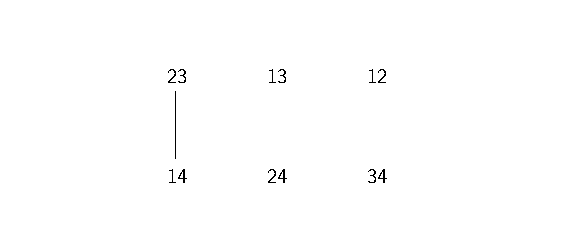
\includegraphics[width = \textwidth]{graph4.pdf}
    The graph $G_5$ is the following
    \\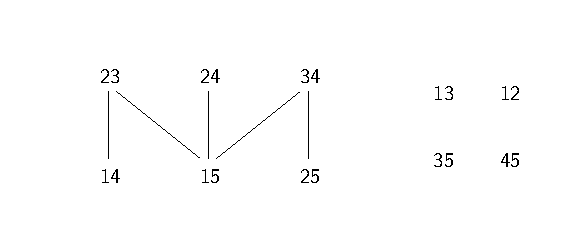
\includegraphics[width = \textwidth]{graph5.pdf}
    The graph $G_6$ is the following
    \\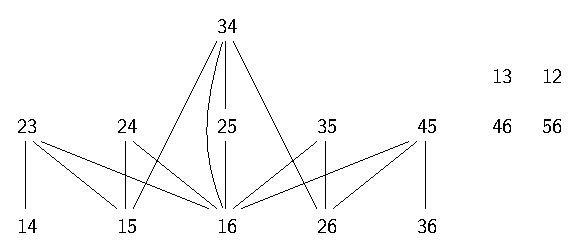
\includegraphics[width = \textwidth]{graph6.pdf}
\end{example}
\begin{lemma}
    The largest independent set in $G_n$ is of size $2n - 3$.
\end{lemma}
\begin{proof}
    The idea is to write the graph in layers (or as a kind of ``pyramid'') as displayed in Example~\ref{ex:Gn}.
    Then we can ``push'' an independent set onto the bottom layer, by repeatedly taking vertices in the set that are maximally high up and on the outside, and replacing them by their ``child''. 
    This shows the claim, as the bottom layer (plus the 4 unconnected vertices, which we also define to be in the bottom layer) has size $2n - 3$.

    Define the ``layer function''
    \begin{equation*}
        l: V \to \N, \quad (i, j) \mapsto \min\{i - 1, n - j\}
    \end{equation*}
    and the ``width function''
    \begin{equation*}
        w: V \to \N, \quad (i, j) \mapsto j - i - 1
    \end{equation*}
    Let $I$ be an independent set that is not contained in the lower layer (i.e. there exists $(i, j) \in I$ with $l((i, j)) > 0$). 
    Define now the compression $C(I) := (I \setminus \{(i, j)\}) \cup \{(i - 1, j + 1)\}$ where $(i, j) \in I$ is a vertex with
    \begin{equation*}
        l((i, j)) = \max_{(a, b) \in I} l((a, b)) \quad \text{and} \quad w((i, j)) = \min_{(a, b) \in I, l((u, v)) = l((i, v))} w((a, b))
    \end{equation*}
    Then clearly $\sum_{\alpha \in C(I)} l(\alpha) < \sum_{\alpha \in I} l(\alpha)$ and we claim that $C(I)$ is an independent set.

    Assume not, i.e. there is $(a, b) \in I \cap C(I)$ such that $\{(i - 1, j + 1), (a, b)\} \in E$.
    As $I$ is independent, find that we cannot have $a < i < j < b$.
    Thus in particular, we have not $a < i - 1 < j - 1 < b$ and so
    \begin{equation*}
        i - 1 < a < b < j + 1
    \end{equation*}
    Since $(a, b) \neq (i, j)$, we either have $a = i, b < j$ or $b = j, a > i$.
    
    In the first case, see that $l((a, b)) = \min\{a - 1, n - b\} \geq \min\{i - 1, n - j\} = l((i, j))$.
    By choice of $(i, j)$, it follows that we must have equality $l((a, b)) = l((i, j))$.
    Since $b < j$ we see that $\min\{a - 1, n - b\} > \min\{i - 1, n - j\}$ unless $\min\{i - 1, n - j\} = i - 1$, so $n - j \geq i - 1$.
    In particular, also $\min\{a - 1, n - b\} = i - 1$ and so $a - 1 = i - 1$.
    It follows that
    \begin{equation*}
        w((i, j)) = j - i - 1 = j - a - 1 > b - a - 1 = w((a, b))
    \end{equation*}
    which is a contradiction to the choice of $(i, j) \in I$ as $l((a, b)) = l((i, j))$.
    The second case can be handled in the same way.

    Now we know that $C(I)$ is an independent set with $\sum_{\alpha \in C(I)} l(\alpha) < \sum_{\alpha \in I} l(\alpha)$.
    Since these sums take values in $\N$ which is well-ordered, we cannot have an infinite sequence
    \begin{equation*}
        I, C(I), C^2(I), C^3(I), ...
    \end{equation*}
    and thus at some point, we find $C^k(I)$ is contained in layer 0.
    Now note that $C$ does not decrease the size, i.e. $|C(I)| = |I|$ and so $|C^k(I)| = |I|$.
    However, there are only $(n - 2) + (n - 2) + 1 = 2n - 3$ elements in layer 0 and we see that there is no independent set of size $> 2n - 3$.

    On the other hand, it is easy to observe that the 0-th layer
    \begin{equation*}
        I = \{ v \in V \ | \ l(v) = 0 \}
    \end{equation*}
    is indeed an independent set, as for all elements $(i, j) \in I$ have either $i = 1$ or $j = n$.
\end{proof}
\begin{corollary}
    Have $\dim(\Gr(2, n)) = 2n - 4$.
\end{corollary}
\begin{proof}
    Follows directly from the previous two statements.
\end{proof}
I also think that it is not too difficult to show that
\begin{equation*}
    s_n(2n - 3) = \frac {(2(n - 2))!} {(n - 2)! (n - 1)!}
\end{equation*}
which then shows the degree formula for the case $d = 2$.
However, this is not a lecture on graph theory or combinatorics, and I already spent a lot of hours on this problem (and there are other mini projects as well :)).
So I will not do the proof here, but I think it is already very interesting to see those graphs and the connection of $\deg(\Gr(2, n))$ to combinatorial problems.
Finally, in the case of $n = 6$ we can simply count the independent sets by hand, and find the following result.
\begin{corollary}[Question (e)]
    Have $\dim(\Gr(2, 6)) = 8$ and $\deg(\Gr(2, 6)) = 14$.
\end{corollary}
\begin{proof}
    The dimension follows directly from the previous general case.
    For the degree, just count the maximal independent sets in $G_6$, as displayed in Example~\ref{ex:Gn}.
    This is slightly tricky, but it is not too hard to see that there are exactly 14 of them.
\end{proof}
Of course, the above statement on $\Gr(2, 6)$ can also easily be found using Computer Algebra.
For example, the following Sage script shows that
\begin{equation*}
    p_{\Gr(2, 6)} = \frac 1 {2880} t^8 + \frac 1 {120} t^7 + \frac {41} {480} t^6 + \frac {39} {80} t^5 + \frac {541} {320} t^4 + \frac {291} {80} t^3 + \frac {3401} {720} t^2 + \frac {101} {30} t + 1
\end{equation*}
from which we easily deduce that
\begin{equation*}
    \dim(\Gr(2, 6)) = 8 \quad \text{and} \quad \deg(\Gr(2, 6)) = \frac 1 {2880} \cdot 8! = 14
\end{equation*}
\lstinputlisting[language = python]{./gr26.sage}
\printbibliography
\end{document}